%!TEX root = ../thesis.tex
\define{\imgpath}{french/img}

\chapter*{Résumé substantiel}
\label{chapter:frecnhresume}
\minitoc

Cette thèse s'intérresse à un problème logique dont les enjeux théorique et pratique sont multiples. Ce problème, dans sa forme simple, peut-être présenté ainsi: Imaginez que vous êtes dans un labyrinthe, dont vous connaissez toutes les routes menant à chacune des portes de sortie. Derrière l'une de ces portes se trouve un trésor; mais vous n'avez le droit d'ouvrir qu'une seule porte. Un vieil homme habitant le labyrinthe connait la bonne sortie et se propose alors de vous aider à l'identifier. Pour cela, il vous indiquera la direction à prendre à chaque intersection. Malheureusement, cet homme ne parle pas votre langue, les mots qu'il utilise pour dire ``droite'' ou ``gauche'' vous sont donc inconnu. Est-il possible de trouver le trésors et de comprendre l'association entre les mots du vieil homme et leurs significations ?

Ce problème, bien qu'en apparence abstrait, est relié à des problématiques concrètes dans le domaine de l'interaction homme-machine et que nous présentons aux chapitres~\ref{chapter:introduction} et \ref{chapter:relatedwork}. En effet, si nous renversons les rôles: un human, prenant la place du vieil homme, souhaite guider un robot vers la bonne sortie du labrytinthe. Ce robot ne sait donc pas en avance quel est la bonne sortie mais il sait oû se trouvent toutes les portes et comment s'y rendre. Imaginons maintenant que ce robot ne comprenne pas a priori le language de l'humain; en effet il est très difficile de construire un robot à même de comprendre parfaitement chaque langue, accent, et préférence de tout un chacun. Il faudra alors que le robot apprenne l'association entre les mots de l'humain et leur sens, tout en réalisant la tâche que l'utlisateur humain lui indique (e.g. trouver la bonne porte). Ce problème n'est pas simple car pour comprendre le sens des signaux il faudrait connaitre la tâche, et pour connaître la tâche il faudrait connaitre le sens des signaux.

Il s'agit donc, pour un labyrinthe donné, de trouver la suite d'action permettant de collecter suffisament d'information de la part de l'humain pour comprendre à la fois le sens de ses mots et la porte derrière laquelle se cache le trésor. Cela dépend donc de la configuration du labyrinthe et de l'historique complet de l'interaction entre les deux protagonistes.

Dans cette thèse nous présentons une solution à ce problème. Pour cela nous faisons dabord l'hypothèse qu'un nombre fini de tâche est défini et connu de l'homme et de la machine, i.e. un nombre fini de portes existe. Nous supposons également que le robot dipose d'un modèle de la logique de l'utilisateur et est donc capable de faire le raisonement suivant: Si l'human veut que j'aille vers la Porte $A$ alors lorsque je suis à l'intersection $I$, il devrait logiquement me dire d'aller dans la direction $D$. Noter que cette phrase commence par une supposition sur la tâche, qui n'est en aucun cas connu à l'avance. Ainsi, le robot étant équipé de plusieurs hypothèses (Porte $A$, $B$, $C$, ..), lorqu'il se trouve à l'intersection $I$, l'utilisateur prononce un mot (e.g. "wadibou"), dont autant d'interpretations sont faite que d'hypothèses sur la tâche.

Notre hypothèse sous-jacente est que l'utilisateur est logique et cohérent tout au long de l'interaction, utilisant ainsi toujours le même mot pour dire la même chose. Il nous faut donc tenir compte de tout l'historique de l'interaction pour analyser quels mots auraient été utilisé pour dire quoi selon chaque hypothèse de tâche. Nous comprenons ainsi que, sous certaine conditions qui sont explicitées au chapitre \ref{chapter:lfui}, il est possible d'éliminer toutes les hypothèses générant des interprétation du sens des signaux incohérentes. L'unique hypothèse restante nous informera donc à la fois de la bonne tâche, i.e. la bonne porte à ouvrir, mais aussi de la bonne association entre les mots de l'utilisateur et les sens qui y sont associés, i.e. du language de l'utilisateur.

Une autre façon de décrire le système présenté dans cette thèse est de parler d'auto-calibration. En effet, en s'adaptant à l'utilisateur pendant l'interaction, notre algortihme ne fait aucun apriori sur le sens des signaux qu'il reçoit. Cela revient bien à créer des interfaces ne nécessitant pas de phase de calibration. Ainsi il peut s'adapter à différentes personnes qui ne parlent pas la même language ou qui n'utilisent pas les mêmes mots pour dire la même chose. Cela veut aussi dire qu'il est facile d'étendre note approche à d'autres modalité d'interaction (e.g. gestes, expression faciales, onde cérébrales) et d'autre domaine d'applications.

% Une personne au capacités de communication réduite doit utiliser une machine pour communiquer avec le monde exterieur, il doit donc pouvoir la commander.

Remplaçont par example du labyrinthe par une tâche plus concrête, plus utile. Prenons example d'une personnes  au capacités de communication réduite avec le monde exterieur. Tel que l'utilisation de fragile clignement des yeux ou en aillant recours à l'enregistremnt de leur ondes cérébrale. Il devient alors difficile, voir même impossible de savoir à l'avance les intentions de communications de ces personnes. Il est donc primordiale de disposer de machine qui sont à même de s'apater automatiquement à chaque personne. Il est donc logique de voir que c'est la communaute de l'interaction cerveau machine qui s'est interresse le plus au problème de l'auto-calibration. En effet, a l'opposé des mode d'interaction classique, telle que la parole, les gestes, ou les expression faciale, nous avons très peu d'apriori sur l'utilisation des signaux du cerveau.

Etrangement, cette thèse ne traite pas directement du problème simple, symbolique, mais s'interresse directement à une représentation non-symbolique des signaux de communications. Ceci dans un but applicatif à court termes auquel de tedieuse preuves mathématiques dans des domaine trop simplifé n'aurait laissé guère de temps à l'experimentation. Ainsi la formulation simple du labyrinthe présenté en début de ce résumé n'est adréssé que dans la toute dernière section de cette thèse par une preuve de la validité de notre solution pour le cas de signaux de communication symbolique et sous de forte contrainte de l'environement.

\subsection*{Résultats}

Notre approche est donc tres génerique et permet à un humain de commencer à interagir avec une machine afin de résoudre une tache sequentiel sans que la machine ne comprenne à l'avance les signaux de communiations de l'utilisateur.

\ref{chapter:bci}
\ref{chapter:lfui}

Nous appliquons nos algortihmes d'auto-calibration à deux examples protypique de l'interaciton homme-robot et de l'interactin cerveau-machine: une tâche d'organization d'une série d'objets selon les préférences de l'utilisateur qui guide le robot par la voix (chapitre~), et une tâche de déplacement sur une grille guidé par les signaux cérébraux (EEG) de l'utlisateur (chapitre~).

\begin{figure}[!htbp]
  \centering
  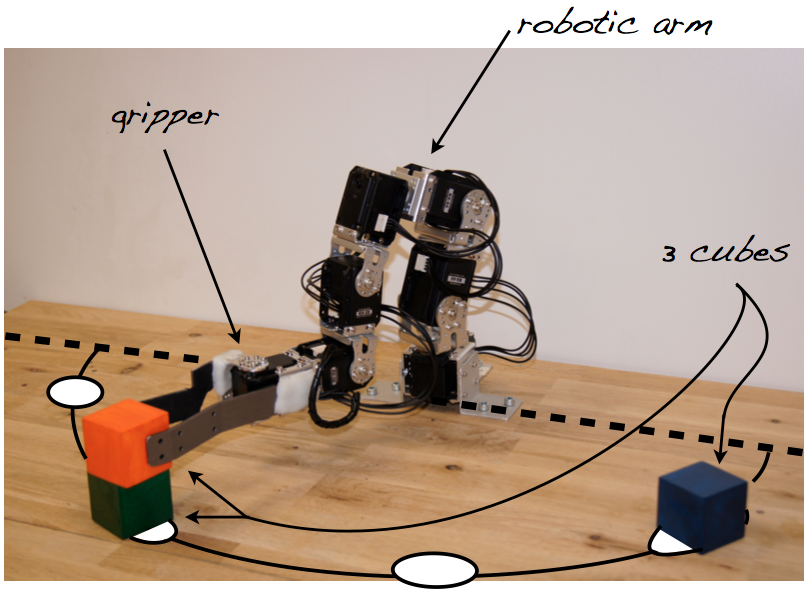
\includegraphics[width=0.49\columnwidth]{chapters/lfui/img/setup.png}
  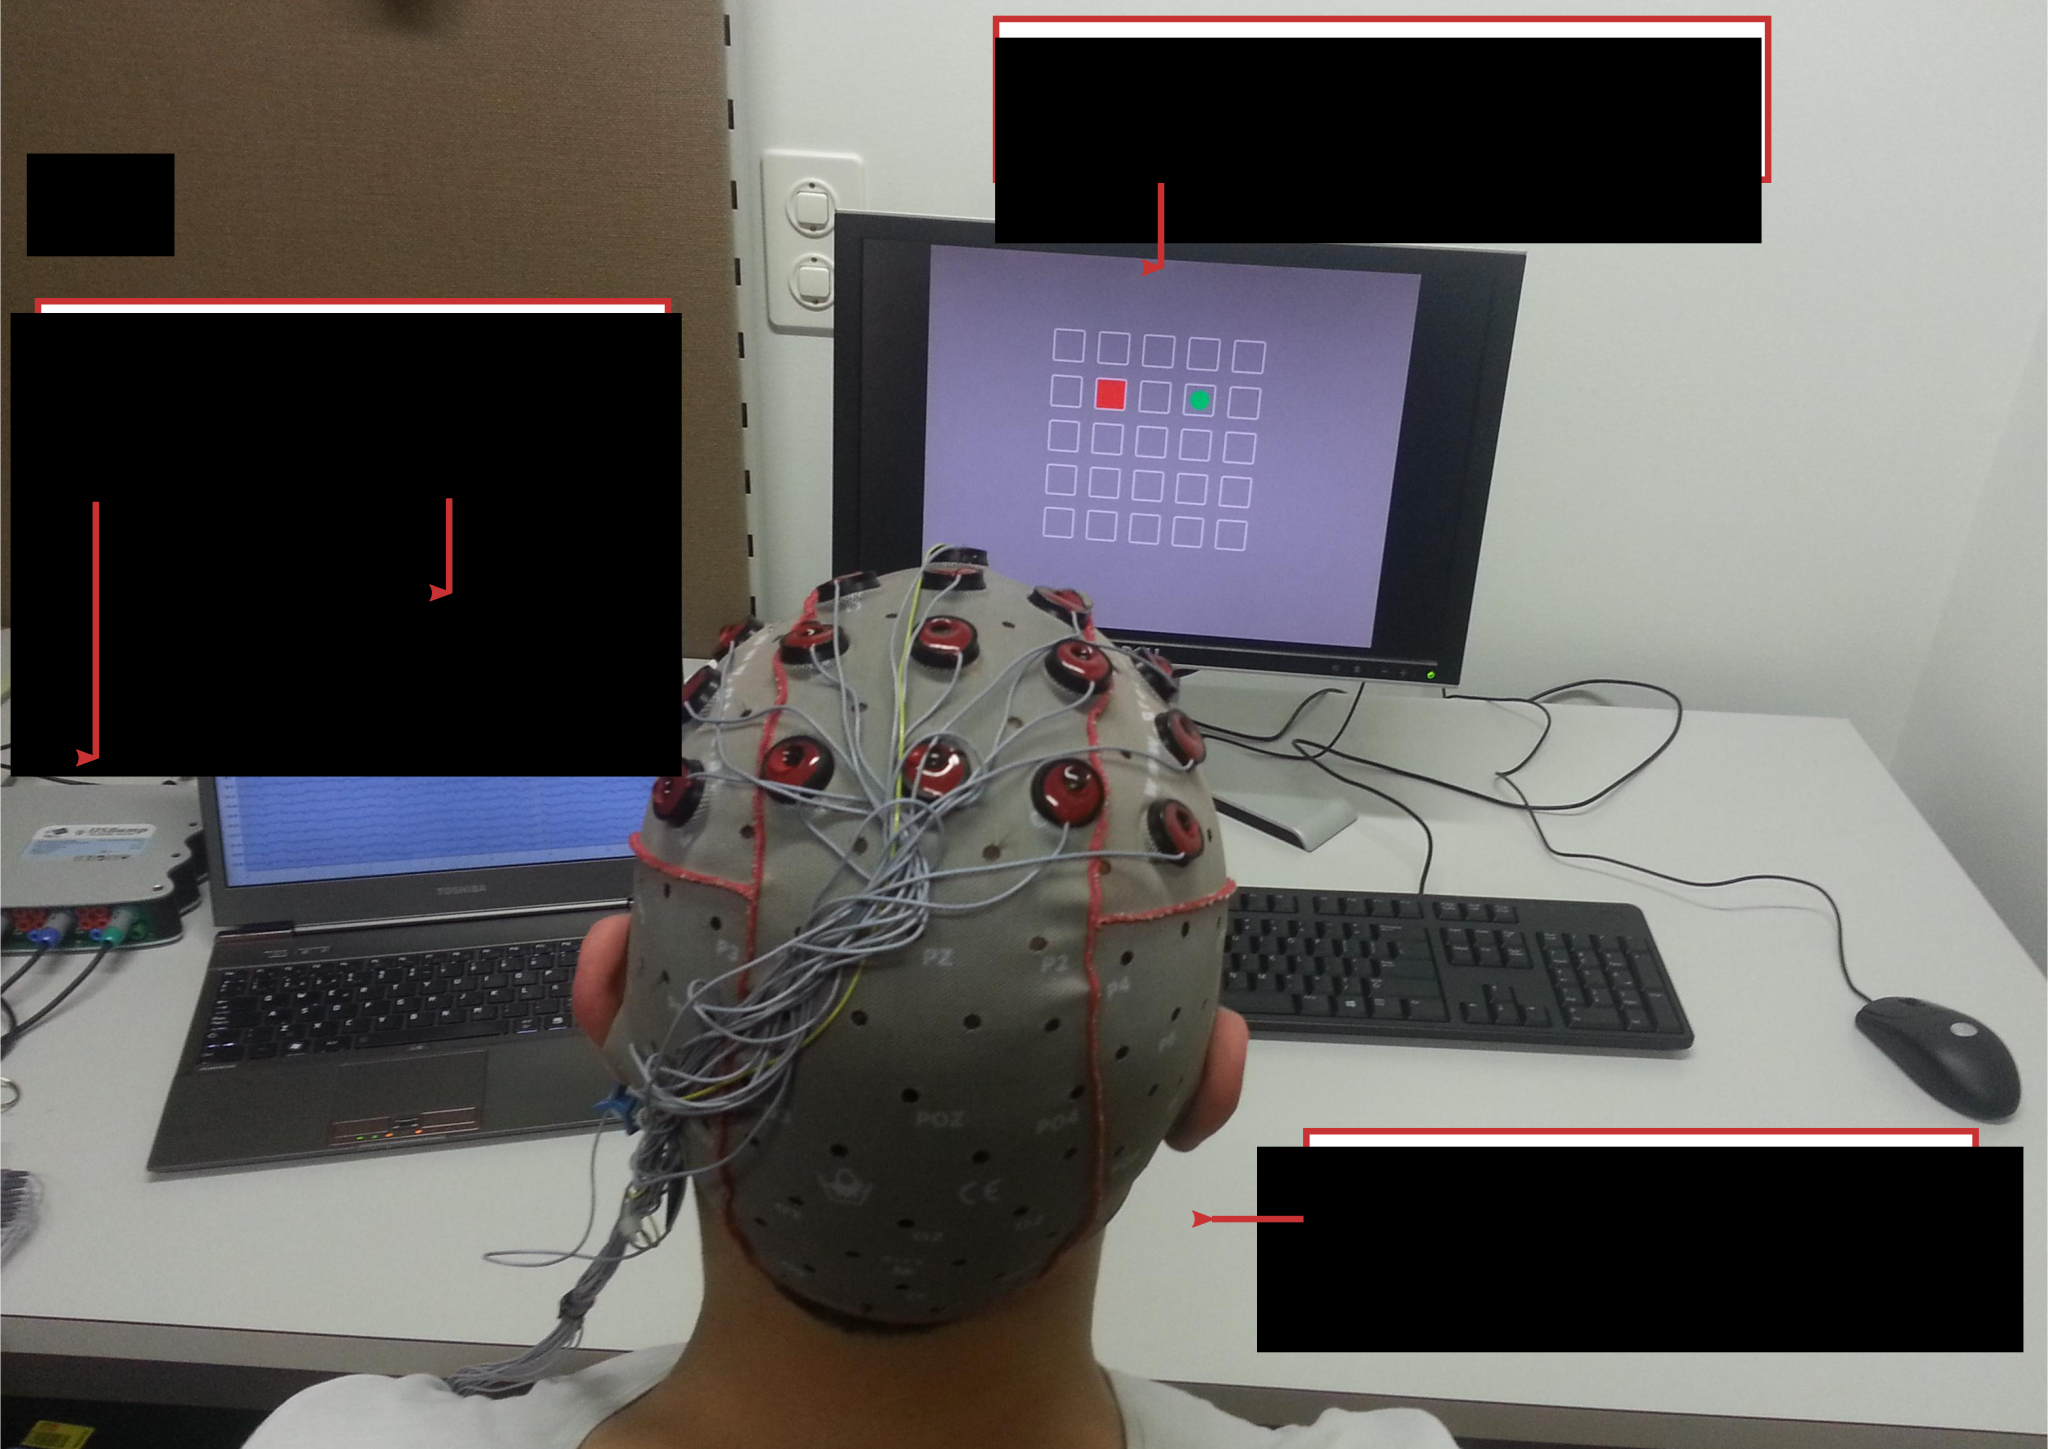
\includegraphics[width=0.49\columnwidth]{\visualspdf/onlineXP/setup.pdf}
  \caption{Illustration des deux setups expérimentaux tangible utilisé dans ce travail. Gauche: Le bras robotique pour la tâche de ``pick and place'' avec trois cubes. Droite: L'interface cerveau machine composée d'un casque avec ces electrodes et d'un ecran affichant les information relative a la tache.}
  \label{fig:setupfrench}
\end{figure}

Bien que les experiences du chapitre sont fondatrice, pour ce bref résumé nous préférons nous concentrer sur les experience BCI qui présente un aspect plus appliqué car testé sur de vrai sujet en temps réel et sur une tâche d'actualitée pour les interfaces cerveau-machine.

Au chapitre bci, nous présentons l'application principale de ce travail au interface cerveau-machine. Ce genre d'interface permet au personne a fort handicap d'interagir avec le monde exterieur par le bias de son cerveau. Plus precisement, nous pouvons enregistrer des varitions de potentiel à la surface du cerveau. Ces ondes ont des porpritété différent en fonction de l'activité mentale du sujet et il est possible de différentier des activité motrice et même des signaux d'erreur de type oui/non. Le problème de ces systeme est qu'ils ne sont pas universelle et doivent être adapté à chaque utilisateur. Ceete adaptation est faite par une periode de calibration ou l'utilisateur, souvent ennuyeuse, et durent laquelle le systeme est inutilisable et neccessitant l'intervention d'une personne exterieur. De plus, cette pahse de calibration doit être effectué régulièrmeent car les signaux varie de jour en jour. Mais aussi pas example lapossition du casqua EEG, necessitant une calibration quotidienne de ce genre d'interface.

Enfin au chapitre \ref{chapter:bci}, nous présentons les résultats d'experiences réel dans le cadre de l'interaction cerveau-machine. Ce sont donc des sujets humanin qui ont pour tâche de guider un agent dans un labyrinthe en lui indiquant si ces actions sont ``correct''  ou ``incorrecte'' vis a vis de l'objectif défini simplement en pensant à ``correct'' ou ``incorrect'' dans leur esprit. Les ``pensées'' de l'utilisateur sont mesuré par le biais d'électrode au contact de son cerveau. Gràce a un procédé décris au chapitre \ref{chapter:bci}, il est possible de représenter ces signaux afin différentier ceux signifiant correct de ceux signifiant incorrect. L'agent ne connait donc ni la tâche à effectuer ni le mapping entre les ondes cérébrales et leur sens (``correct'' ou ``incorrect'').

La figure~\ref{fig:sequencefrench} presente le résultat principle de cette thèse. Elle compare la différence entre un algorithme nécessitant une pahse de claibration et les algortihme de self-calibration développé dans cette thèse.  Ce sont des résultats de simulation avec des donnée EEG réelle. Notre algortihme (haut) permets de résoudre une première tache en seulement 85 itérations, bien avant que la phse de calibration ne soit complète (400 itérations étant un durée normale de calibration pour ce genre de système).
Enfin notre méthode résoud une dixaine de tache en 400 itérations, soit avant qu'un système traditionnel ne soit opérationnel. Les même expèriences on été testé avec des utlisateurs réel. Leur résultats confirme les résultat de simulation et sont présenté au chapitre \ref{chapter:bci} ainsi qu'au chapitre \ref{chapter:limitations:overlap}.

\begin{figure}[!htbp]
\centering
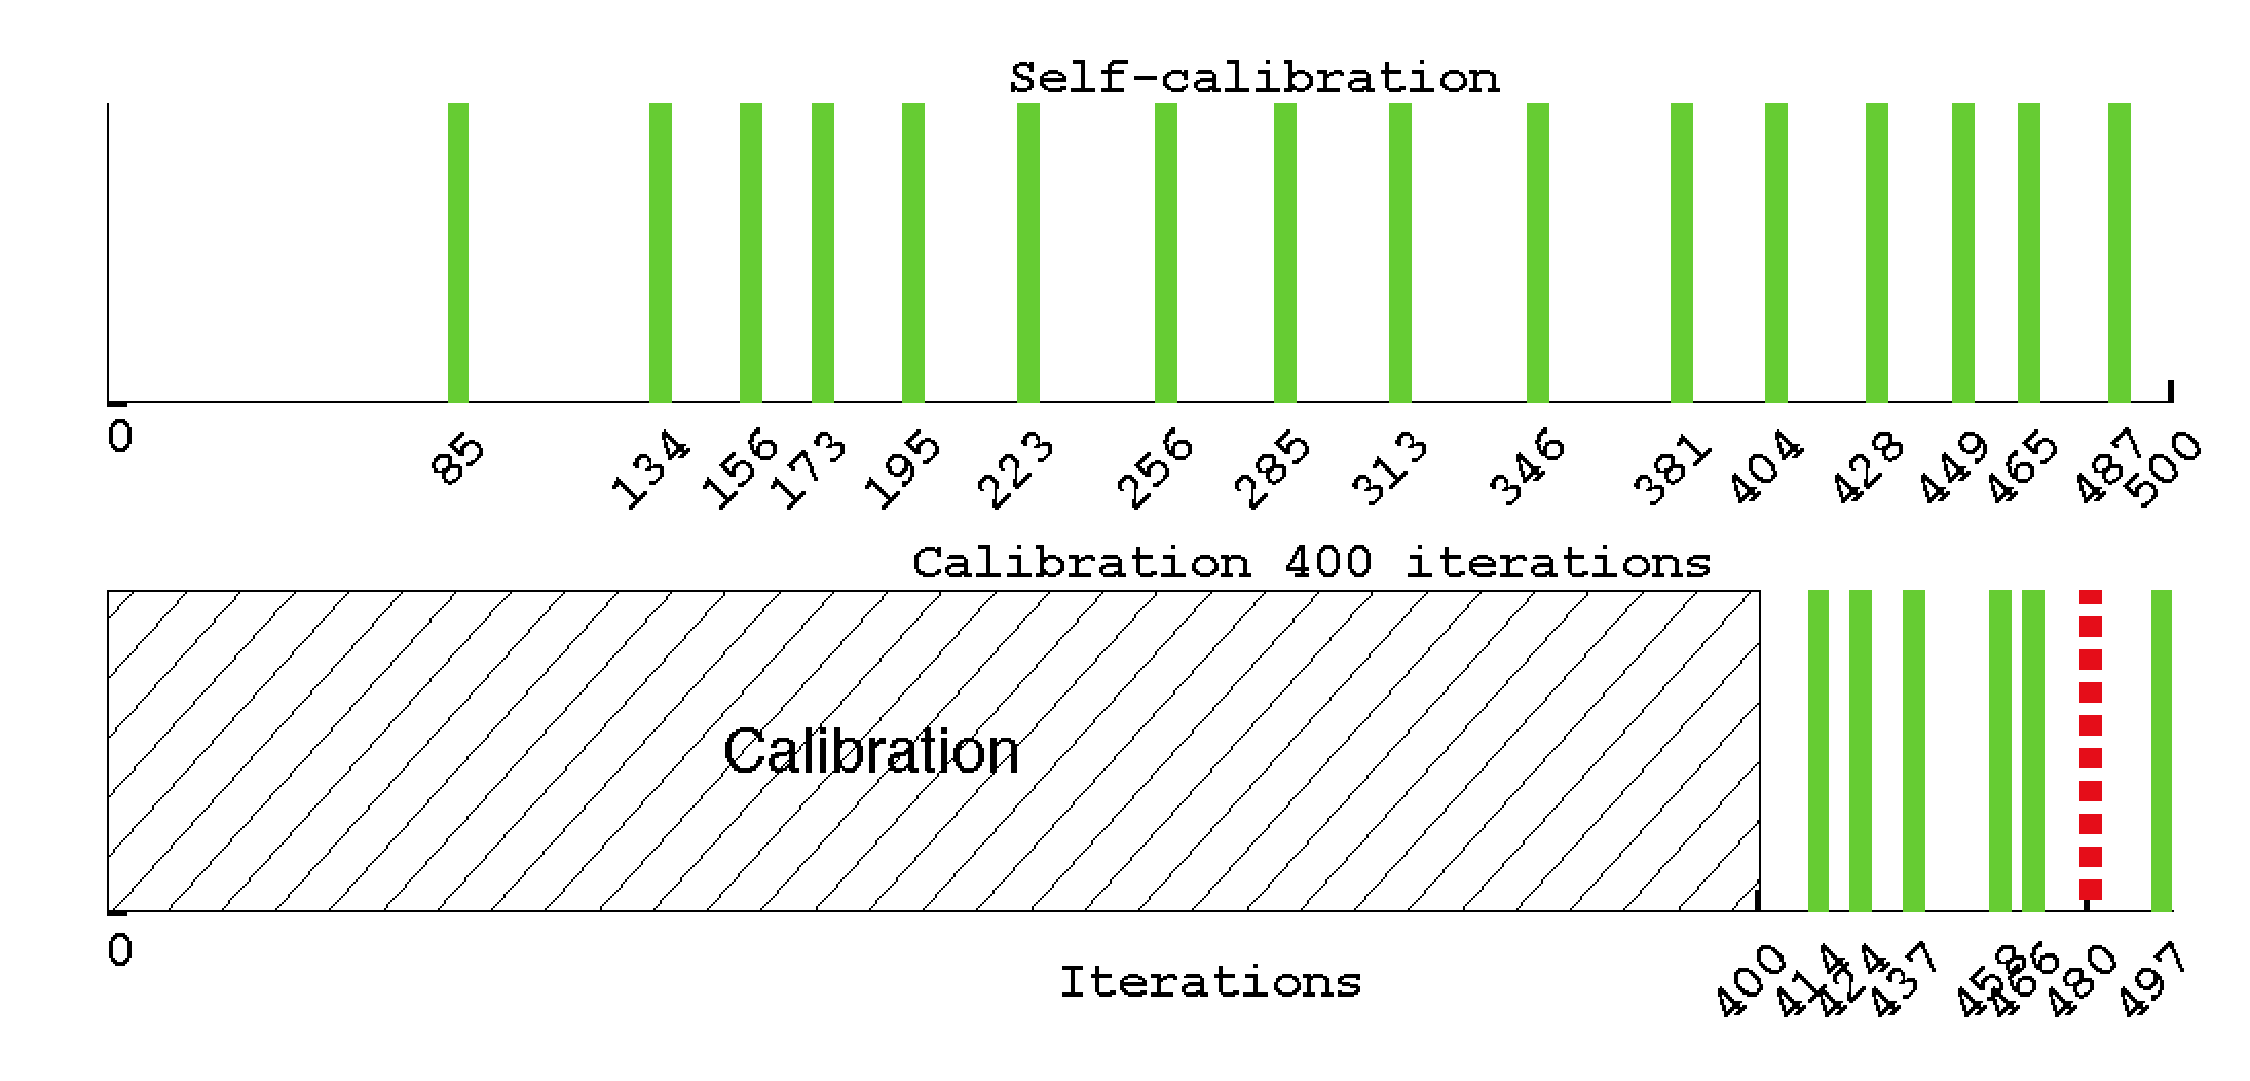
\includegraphics[width=\sequencesize\columnwidth]{\imgpath/plot_the_aaai_sequence.eps}
\caption{Nombre de tâche résolue dans le temps avec des données EEG. L'algortihme d'auto-calibration (haut) est comparé au methode nécessitant une phase de calibration (bas, ici 400 itérations de calibration. Le barres verte et rouge represente respectivement les bonnes et les mauvaise executions de la tàche par la machine. La méthode de'auto calibration proposé dans cette thèse permet de completer une premiere tache plus rapidement, sans pour autant faire d'érreur.}
\label{fig:sequencefrench}
\end{figure}

Finalement, le planning est égelement différent des algortihmes précedemment dévellopé. En effet une couche d'incertitude supplémentaire est présente, le sens des signaux est inconnue et nous disposont d'une multitude de candidat possible. Il faut donc inclure cette incertitude dans la mesure d'incertidtude globale permettant de naviguer plus efficacement dans le monde. afin de collecter des signaux varié.

Les resultate presente au chapitre montre que notre methode de planification des actions ameliroe significativement le temps nécessaire à l'identification de la tâche mais aussi à l'établissement du modèle de language de l'utlisateur.
\ref{chapter:planning}

Nos résultats montre que notre approche est fonctionnelle et permet une utilisation pratique de l'interface plus rapidement. De plus notre systemem ne necessite pas la presence d'une personne exterieur pour calibraiton le système et est donc un candidat potentiel pour ammener l'utilisation des interface cerveau mahcine dans les maisons.


\subsubsection*{Extensions}

\ref{chapter:limitations:continousstate}
\ref{chapter:limitations:continuoushypothesis}
\ref{chapter:limitations:framehypothesis}
\ref{chapter:limitations:proof}


Au chapitre~\ref{chapter:limitations}, nous abordons et porposons des solutions à de multiples limitations de l'approche présentée dans cette thèse. Nous montrons d'abord qu'il est possible d'utiliser le systeme dans des espaces continue: premièrement pour un état continue du système mais sur un ensemble infini d'hypothèse sur la tâche. Par la suite, nous montrons que la connaissance a priori du protocole d'intéraction n'est pas une limitation forte et que notre systeme peut détecter le protocole par l'interaction pratique avec l'utlisateur. Finalement, nous démontrons mathematiquement sur un example simplifié et sous certaine conditions que notre méthode est garanti d'identifier la bonne hypothèse. Ce dernier dévelopement montre que ce genre de problème peut-être modélisé mathématiquement et ouvre la voie de prochaine exploration plus théorique de ce problème. Permettant peut-être de trouver des  guarantie plus grande sur la convergence et les performance de nos algorthmes. Bien que ce genre de preuve semble encore très limité pour l'interaction pratique de par la nature imprevisible du comportement humain.

\subsection*{Expèrience humain-humain}

\ref{chapter:humanexperiment}

Une autre contribution de cette thèse et la mise en place d'un protocol experimental pour analyser le comportement de deux humain mis dans la situation que doivent résoudre nos algorithmes. Dans cette expèriences deux humains doivent collaborer à l'execution d'une tâche de construction. Il s ne peuvent intéragir que par le biais d'une interface dont le sens des signaux transmis est inconnu et indefini au départ pour les deux parties.

Il est intérressant de voir la dynamique de construction d'un language commun entre les deux participants. Language qui n'était pas prévu au début de l'interaction s'établi de tel sorte qu'une personne extèrieure à l'experience ne pourra alors pas comprendre ce qui ce passe en observant le résultat final de l'intéraction.

\subsection*{Conclusion}

La vision dévellopée dans cette thèse est qu'il est possible pour une machine d'intéragir avec un humain sans comprende a priori la façon dont l'utisateur communique l'information. Plus concretement notre systeme n'a pas d'apriori sur le sens des signaux reçu et construit son modèle durant l'interaction pratique avec l'utilisateur sans jamais avoir access a une source sûre d'information. Cela sera, nous l'espèrons, le fruit de nombreux travaux futur.

Au dela du challenge technique de l'auto-calibration, des questions d'utilisation pratique et d'acceptabilité éclosent et sont presentées au chapitre~\ref{chapter:limitations:userstudies}. Parmis elle, la plus important à tester en condition réelle est: Comment les utlisateurs vont réagir au fait que la machine, le robot, ne soit pas immédiatement réactif à ces ordres mais doivent apprendre le sens des signaux pendant l'interaction? En effet, même si nos algortihmes apportent une plus grande flexibilité d'intéraction, ils ne permettent pas à l'utilisateur une fonctionalité parfaite et immmediate du système qui doit donc apprendre de l'interaction. Cette ephase d'apprentisssage pourrait être percus comme une inopérabilité du système et par conséquent impacter interet et l'utilisabilité réelle de notre sytème.\\

\noindent {\large\textbf{Mots-clés:}} Auto-Calibration, Apprentissage par interaction, Intéraction Human-Robot, Interface Cerveau-Machine, Intéraction Intuitive et Adaptative, Robotique, Acquisition de Symbole, Apprentissage Actif, Calibration.\\

Ce travail a été financé par INRIA, le Conseil R\'egional d'Aquitaine et la bourse ERC EXPLORERS 24007.
